\subsection{Pengujian Komponen \textit{Metrics Fetcher}}

Pada bagian ini akan dijelaskan tentang tujuan, skenario, hasil, dan analisis dari pengujian komponen \textbf{\textit{Metrics Fetcher}}.

\subsubsection{Tujuan Pengujian}

Tujuan pengujian ini memastikan komponen \textbf{\textit{Metrics Fetcher}} dapat berjalan dengan baik dan menghasilkan data yang sesuai dengan ekspektasi.

\subsubsection{Skenario Pengujian}

Pengujian terhadap komponen \textbf{\textit{Metrics Fetcher}} dilakukan dengan beberapa skenario sebagai berikut serta ekspektasi dari pengujian yang dilakukan.
\begin{enumerate}
    \item \bfseries\textit{Elastic Search} sedang \textit{idle}.\normalfont
    
        Data yang diminta dari \textit{Node Stats API} diekspektasikan relatif statis dan berhasil diletakkan pada \textit{stream file}.
    \item \bfseries\textit{Elastic Search} sedang digunakan untuk melakukan operasi penambahan data.\normalfont
    
        Data yang diminta dari \textit{Node Stats API} seharusnya relatif berubah terutama pada aspek \textit{throughput} operasi \textit{index} dan \textit{bulk}. Lalu, data tersebut diekspektasikan berhasil diletakkan pada \textit{stream file}.

    \item \bfseries\textit{Elastic Search} sedang digunakan untuk melakukan operasi pencarian data.\normalfont
    
        Data yang diminta dari \textit{Node Stats API} seharusnya relatif berubah terutama pada aspek \textit{throughput} operasi \textit{query} dan \textit{fetch}. Lalu, data tersebut diekspektasikan berhasil diletakkan pada \textit{stream file}.
\end{enumerate}

\subsubsection{Hasil Pengujian dan Analisis}

Hasil untuk skenario 1 dapat dilihat pada gambar \ref{fig:mf-1}. Data yang ditarik sudah relatif statis untuk semua aspek dan berhasil diletakkan pada \textit{stream file}. Untuk skenario 2, dapat dilihat pada gambar \ref{fig:mf-2}. Data yang ditarik sudah mengalami perubahan pada operasi \textit{index} dan \textit{bulk} serta berhasil diletakkan pada \textit{stream file}. Terakhir, skenario 3, dapat dilihat pada gambar \ref{fig:mf-3}. Data yang ditarik sudah mengalami perubahan pada operasi \textit{query} dan \textit{fetch} serta berhasil diletakkan pada \textit{stream file}.

\begin{figure}[h]
    \centering
    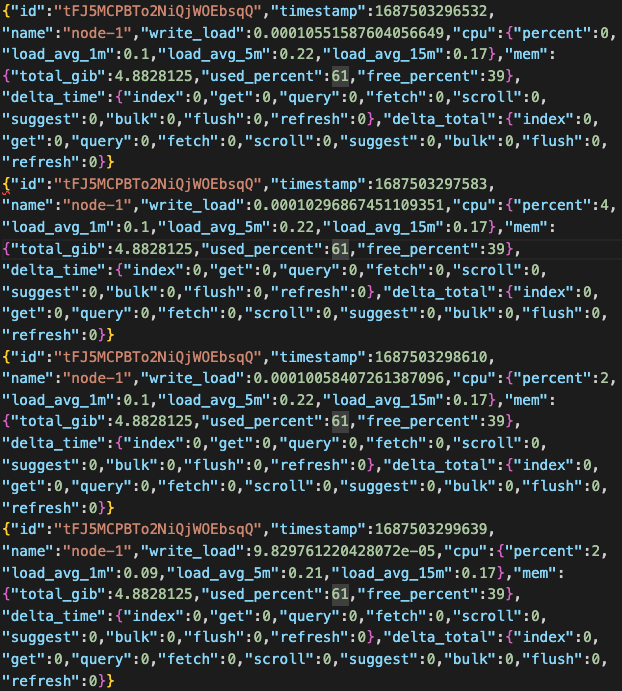
\includegraphics[width=0.8\textwidth]{chapter-4/mf-1.png}
    \caption{Hasil Pengujian Komponen \textit{Metrics Fetcher} Skenario 1}
    \label{fig:mf-1}
\end{figure}

\begin{figure}[h]
    \centering
    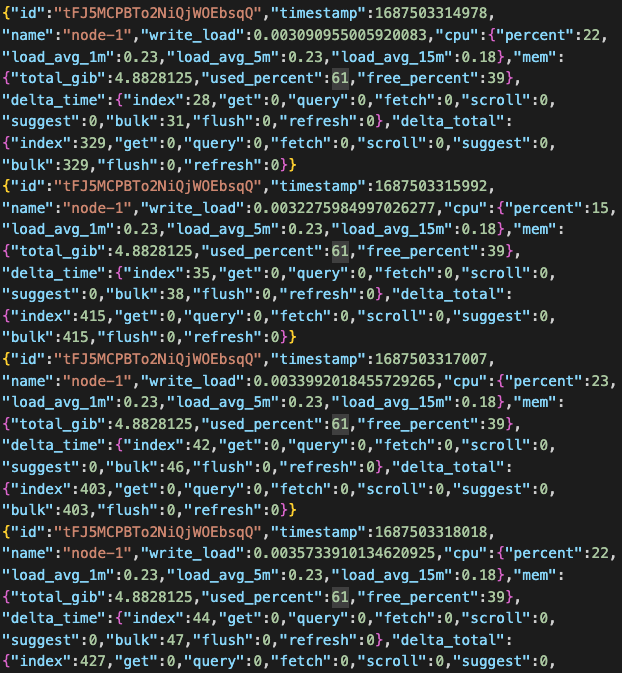
\includegraphics[width=0.8\textwidth]{chapter-4/mf-2.png}
    \caption{Hasil Pengujian Komponen \textit{Metrics Fetcher} Skenario 2}
    \label{fig:mf-2}
\end{figure}

\begin{figure}[h]
    \centering
    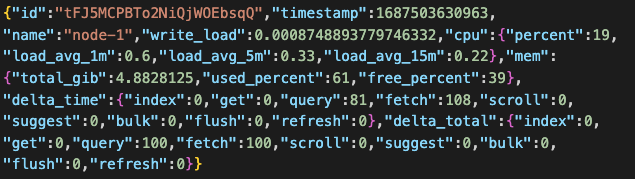
\includegraphics[width=0.8\textwidth]{chapter-4/mf-3.png}
    \caption{Hasil Pengujian Komponen \textit{Metrics Fetcher} Skenario 3}
    \label{fig:mf-3}
\end{figure}

Pengujian komponen \textbf{\textit{Metrics Fetcher}} sudah sesuai ekspektasi dan dapat dilanjutkan ke pengujian komponen lainnya.